\section{Risk Management}

\subsection{Risks}

\begin{table}[!ht]
    \makebox[\textwidth][c]{
        \begin{tabular}{ p{2cm} p{8.15cm} p{2cm} p{2cm}}
            \textbf{Risk Nr.} & \textbf{Description} & \textbf{Probability} & \textbf{Severity} \\ \hline \\                                                                                                                                                                           
            \textbf{R1} & Unfamiliar Technology (f.ex. Haskell Core) & 2 & 3 \\
            \textbf{R2} & Sickness & 1 & 2 \\
            \textbf{R3} & Goals set too high (too many or too complex features) & 2 & 1\\
            \textbf{R4} & Infeasibility of CLI Tool (not enough interactiveness) & 1 & 4\\
            \textbf{R5} & Infeasibility of GUI Tool (build too complex) & 2 & 1\\
            \textbf{R6} & Tool is too complicated (usability) & 1 & 3\\
            \textbf{R7} & Missing functionality of core stepper & 1 & 2\\
        \end{tabular}
    }
    \caption{Identified Risks in the Project}
    \label{tab:risks}
\end{table}

The identified risks can be visualized in the following risk matrix (Table \ref*{tab:risks}).

\begin{figure}[!ht]
    \centering
    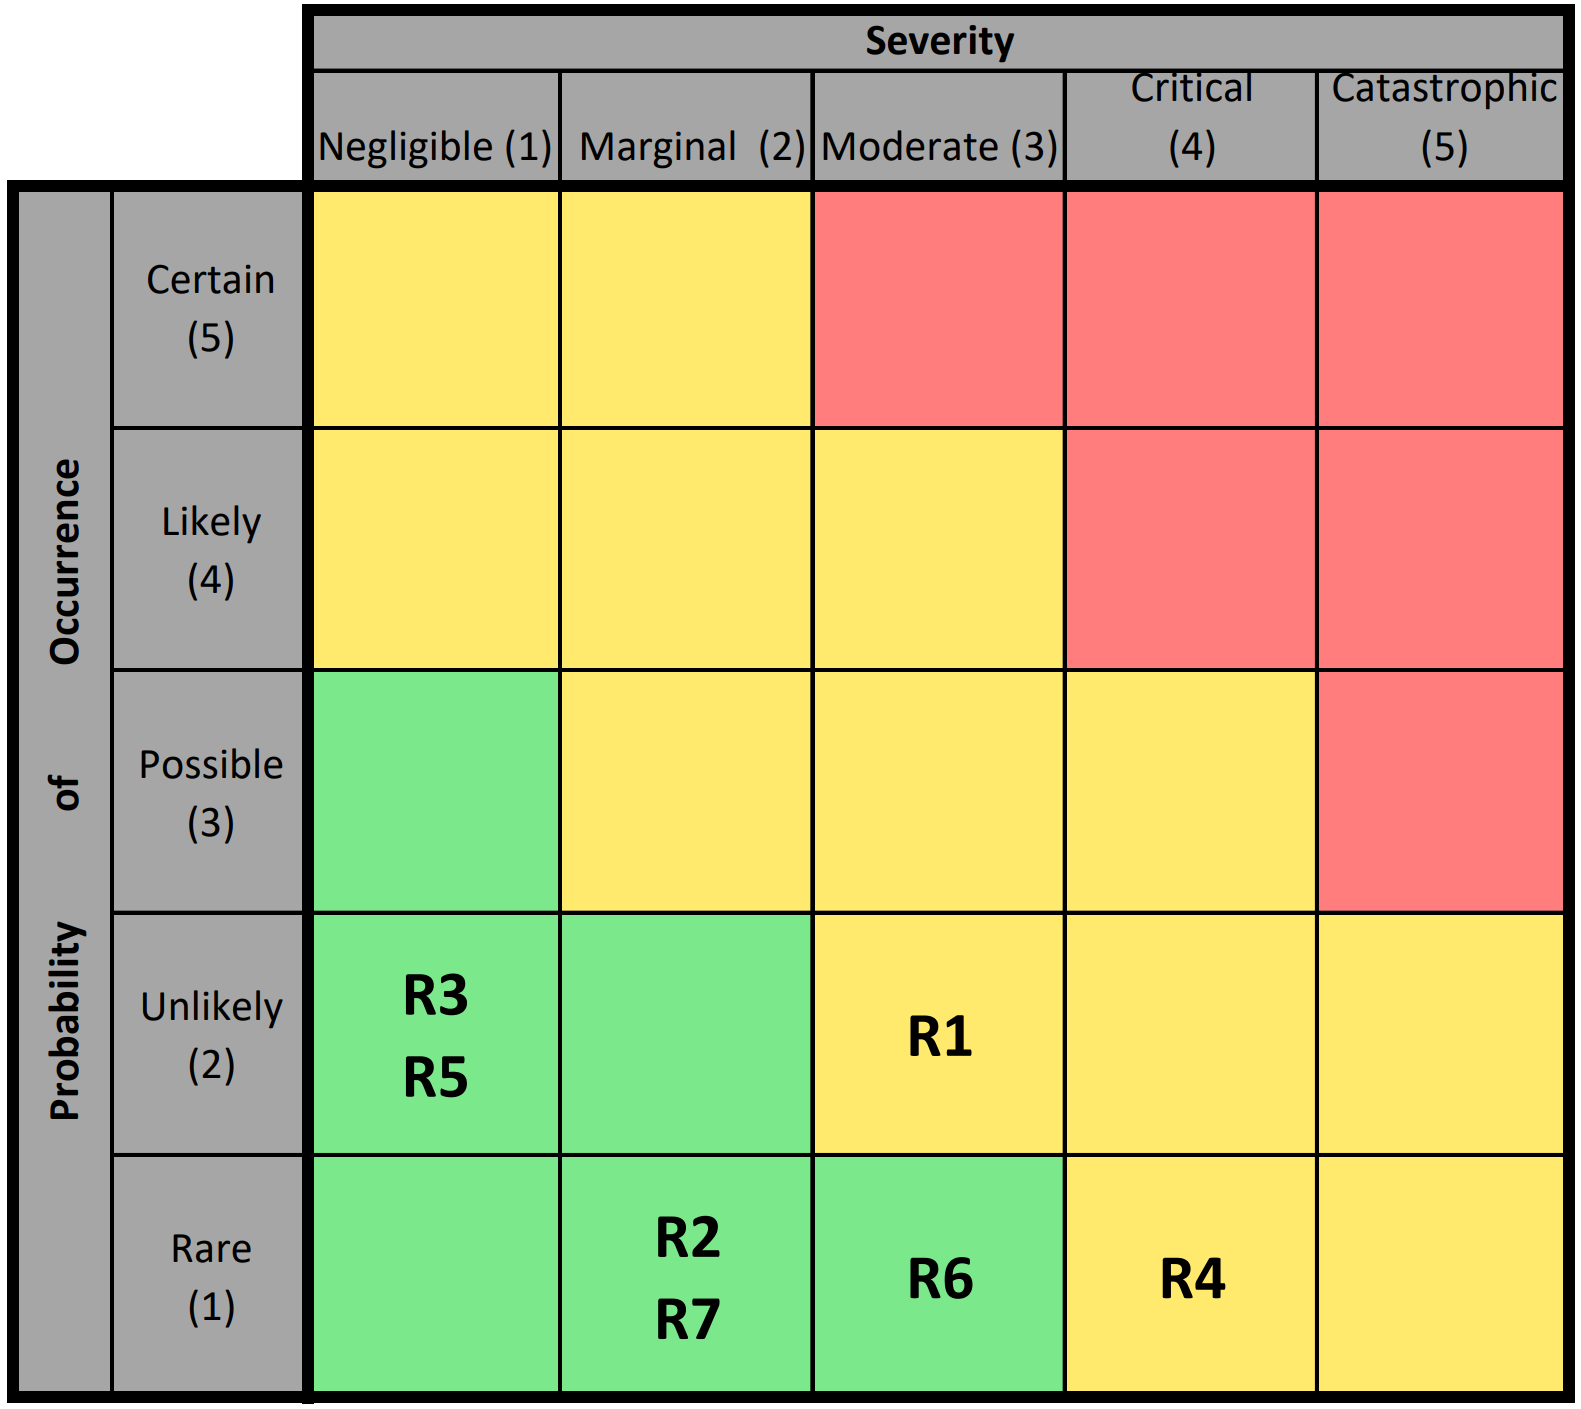
\includegraphics[width=0.6\textwidth]{resources/RiskMatrix.PNG}
    \caption{Risk Matrix}
    \label{fig:riskMatrix}
\end{figure}

\subsection{Mitigations}

In case one or more of the listed risks arise and turn into issues,
there is mitigations in place in order to reduce the severity of these issues.
These mitigations are shown in \ref*{tab:mitigations}.

\begin{table}[!ht]
    \makebox[\textwidth][c]{
        \begin{tabular}{ p{2cm} p{12.15cm}}
            \textbf{Risk Nr.} & \textbf{Mitigation} \\ \hline \\                                                                                                                                                                           
            \textbf{R1} & Robin and Lukas can be consulted in case there is any problems with existing software. \\
            \textbf{R2} & A time buffer at the end of the project is set in place, in case of sickness. \\
            \textbf{R3} & A time buffer at the end of the project is set in place, in case the estimates are too low. \\
            \textbf{R4} & A proof of concept is done at the start of the project. If it doesn't meet the requirements, a switch to a GUI could be done. \\
            \textbf{R5} & The GUI tool is not an essential feature and can thus be omitted. \\
            \textbf{R6} & Definition of an NFR that keeps the usage as simple as possible. \\
            \textbf{R7} & A time buffer at the end of the project is set i nplace, in case some functionality needs to be added in the core stepper. \\
        \end{tabular}
    }
    \caption{Mitigations for the identified risks.}
    \label{tab:mitigations}
\end{table}
